\documentclass[]{article}
\usepackage[hidelinks]{hyperref}
\usepackage{graphicx}
\usepackage[inline]{enumitem}
\usepackage{listings}
%opening



\begin{document}

\begin{flushleft}
\centering\LARGE {\bf Comparative Evaluation of Spark and Flink Stream Processing}

Supervisor: PD Dr. Michael Mock
\thispagestyle{empty}
\end{flushleft}
\newpage
\tableofcontents

\newpage


\begin{abstract}

\end{abstract}
Recent years have witnessed a big development improvements of Big Data frameworks such as Apache Spark and Apache Flink. For example, both frameworks support real-time
streaming processing. While which platform is the best still an open question. 
In this paper, we provide a performance comparison of streaming data processing in Apache Spark and Apache Flink, by measuring different performance metrics, namely latency and throughput. In addition, we cover some key aspects of streaming data applications and how they are handled in both frameworks. The experiment is done using multiple streaming workloads over real-world datasets.
\section{Introduction}

\par In recent years, Big Data is considered as one of the most appealing topics in Information Technology, it has gained increasing attention of professionals in industry and academia, as a result of the fact that the amount of data we generate is increasing exponentially \cite{idc} that generated from social media platforms, mobile phones, IoT and finical transactions, etc. Moreover, recent years showed a rapid development of Big Data frameworks such as Apache Spark and Apache Flink that provide more and efficient data processing capabilities.
 \par The Big Data is a method to process not just only large datasets (volume), but also the data that arrives in high rate (velocity), and it comes in all kinds of data format (variety) (i.e., 3Vs of Big Data (Volume, Velocity, Variety)) \cite{svs}.

\par The processing models of Big Data are Batch processing and Stream processing, Batch processing is a way to handle large, finite volumes of data (e.g., processing of historical transaction records), is more concerned with throughput. While the Stream processing  is a method to manage fast and continuously incoming data (real-time), process it as it arrives (e.g., credit card fraud detection and network monitoring applications), where the low latency is required. The variety of data (structured and semi-structured) is included in the two processing models.

\par The are some performance evaluation of Apache Spark and Apache Flink and other framework such as Yahoo Streaming Benchmark \cite{yahoo}. We believe that we still need to carry our evaluation for two reasons: \begin{enumerate*}[label=(\roman*)]
\item both frameworks are continuously improving in short time 
\item we aim to study the performance of some complex operations such as \texttt{groupByKey} \& \texttt{keyBy} in Apache Spark and Apache Flink, respectively.
\end{enumerate*}

 

\par The purpose of this paper is to provide a comparative experimental evaluation of throughput, latency (i.e., performance) of stream processing in Apache Spark and Apache Flink. We use a datasets of airplanes trajectories provided in the context of Datacron project\footnote{\url{http://www.datacron-project.eu/}}, in order to simulate real-world use cases. Using multiple streaming data workloads. Also we try to cover general aspects of streaming processing tasks (later details in Section 3) and how they can be solved in each platform. Informally,  this work aims to help the developers to determine which platform to choose in production for different use cases. 


\par The remainder of this paper is organized as follows.
In Section 2, we present the main characteristics, APIs, and main data abstraction of Apache Spark and Flink. Section 3  presents the general aspects of streaming processing, the design and implementation of experimental workloads. Section 4
provides and compares the performance results of the different workloads. Finally, Section 5 gives the overall conclusion.

\section{Technical Background}
 In this section, we present the architecture, key characteristics, programming APIs  of Apache Spark and Apache Flink. Moreover, a brief overview of the Apache Kafka platform is  provided.

\subsection{Apache Spark}

\par Apache Spark is an open source project that provide general framework for large-scale data processing \cite{spark}. It offers programming API in Java, Scala, Python and R. Its stack includes set of built-in modules including Spark SQL, MLlib for machine learning, GraphX for graph processing, and Spark Streaming to process real-time data streams. It can access different data sources including Hadoop Distributed File System (HDFS), Apache Cassandra database, Apache HBase database etc.

\par The main data abstraction in Spark core is the Resilient Distributed Datasets (RDDs), which is in-memory collection of elements partitioned across cluster of computers that can be processed in parallel \cite{rdd}. RDDs supports two categories of operations: transformations that drive new RDDs from the operated ones (e.g., map), and actions which return a certain value (e.g., count). On the other hand, the Discretized Stream (DStream) is the data abstraction in Spark Streaming, which is series of RDDs that represent an input stream of data \cite{spark_streaming}. In other words, the Spark Streaming is batch-based processing model, which process the continuous stream of data by divided into micro-batches to be processed by the Spark engine. Figure 1 illustrates the general process flow of Spark Streaming. 


\begin{figure}[h]
 
  \centering
    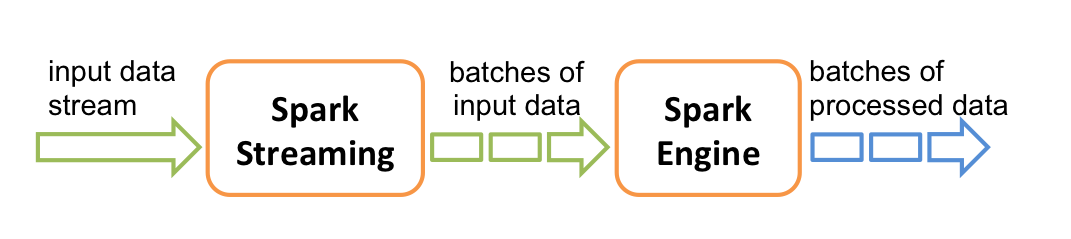
\includegraphics[width=.9\textwidth, height=.2\textheight]{streaming-flow.png}
     \caption{ Process flow of Spark Streaming \cite{spark_streaming}.}
\end{figure} 

\subsection{Apache Flink}

\par Apache Flink is an open source project that provide large-scale, distributed stream processing platform, while the batch processing treated as special case of streaming applications (i.e., finite stream)  \cite{flink}.
It offers programming API in Java and Scala. Its software stack includes the core DataStream and DataSet APIs with additional libraries such as Complex event processing for Flink (FlinkCEP), Machine Learning for Flink (FlinkML), and Flink Graph API (Gelly).

\par The main data abstraction of Flink are DataStream and DataSet that represent read-only collection of data elements. The list of elements is bounded (i.e., finite) in DataSet, while it is unbounded (i.e., infinite) in case of DataStream.

\par The Flink's core is a distributed streaming dataflow engine,  each Flink program is represented by a data flow graph (i.e., directed acyclic graph - DAG) that executed by the Flink's engine \cite{flink_paper}. The data flow graphs are composed of stateful, parallel operations and intermediate data stream partitions. Figure 2 shows a data flow graph of Flink program.


\begin{figure}[h]
 
  \centering
    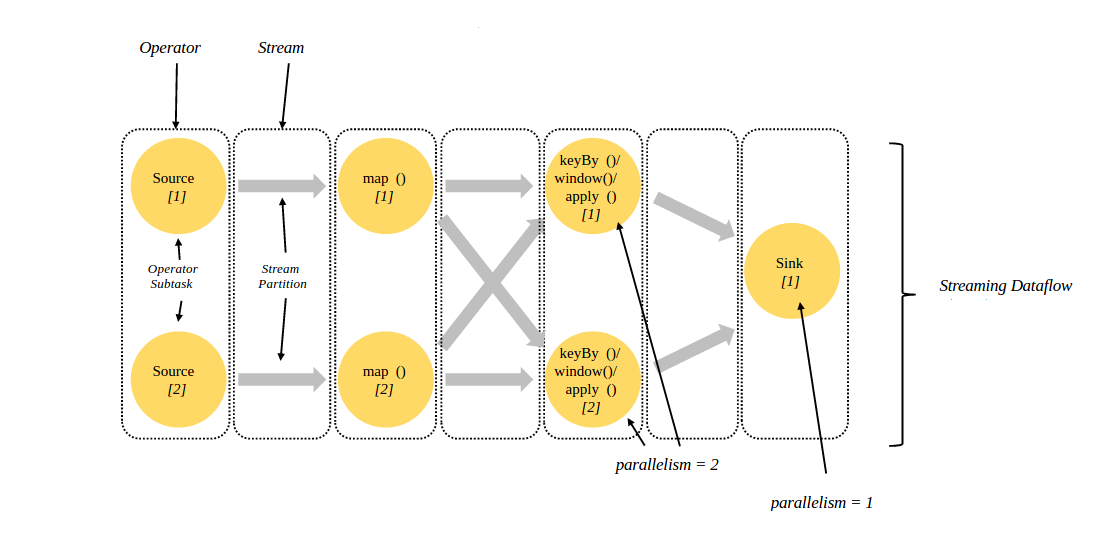
\includegraphics[width=\textwidth, height=.4\textheight]{flink_engine.png}
     \caption{ An example of data flow graph \cite{flink}.}
\end{figure} 
\subsection{Apache Kafka}
\par Apache Kafka is scalable, fault-tolerant distributed publish/subscribe streaming framework \cite{kafka}.
It manges the stream records in different categorizes (i.e., topics) that portioned and distributed over the servers of the Kafka cluster. It allows the data producers to publish stream of records to certain Kafka topic. While the consumer applications can subscribe to one or more topic to read the data stream. The consumers are grouped into groups based on the group name that allows Kafka to distribute and balance the stream partitions among the  members of a certain group for the sake of scalability. Figure 3 shows how 4 partitions of stream is distributed differentially between two groups of consumers based on the number of members. 
Apache Kafka has been widely  adopted, for example, 
Spark and Flink can receive data stream from Kafka. 

\begin{figure}[h]
 
  \centering
    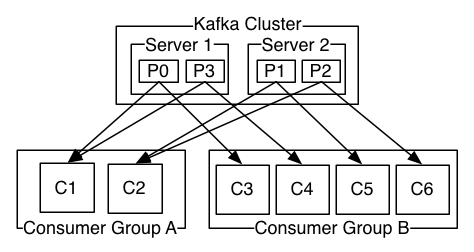
\includegraphics[width=\textwidth, height=.3\textheight]{kafka_groups.png}
     \caption{ Distribution of stream partitions for consumer groups in Kafka \cite{kafka}.}
\end{figure} 

\section{Experiment Setup and Implementation}
This section describes the data stream setup, design of evaluation streaming workloads, and implementation details in Spark and Flink.

\subsection{Data Stream Setup}
Our streaming workloads read input data stream from Kafka. In order to simulate real-world uses cases we use datasets of Automatic Dependent Surveillance – Broadcast (ADS-B) messages that present the aircraft's position over time, comprise 22 fields of data such as aircraft ID, date message generated, longitude, latitude, and altitude.
\par In our experiment a data stream producer component reads the ADS-B datasets, then publish it to Kafka cluster to be consumed by the workloads in Spark and Flink. Figure 1 illustrates the data producer and the Kafka cluster setup.
The data stream is portioned into four portions over two server, while the data producer publish the stream records randomly to Kafka partitions.

\begin{figure}[h]
 
  \centering
    \includegraphics[width=.9\textwidth, height=.2\textheight]{kafka.png}
     \caption{Data Stream Producer \& Kafka Cluster Setup.}
\end{figure} 

\subsection{Evaluation Streaming Workloads}
In our experimental evaluation, we developed two real-time stream processing workloads that read the ADS-B messages stream from Kafka in order to perform basic trajectories analysis methods. The workloads are designed in such way that cover general key aspects of real-time streaming processing tasks, and evaluate the corresponding solutions in Spark and Flink. The following are the aspects of streaming data processing were covered by our workloads's design: 

\begin{itemize}
\item Handling parallel input streams (e.g., Kafka Stream).
\item How to aggregate the state of input stream.
\item Manage the order of stream records.
\item How to provide and update global data model in stream processing task.
\item Evaluate the performance by measuring  the latency and throughput.
\end{itemize}
We present the description of workloads and the relation with these aspects, and th implementation details of Spark and Flink solutions in Section 3.2.1 \& 3.2.1. Afterward, In Section 4 we discuss the performance evaluation and analysis of workloads.

\subsubsection{Statistics Computation per Trajectory}
In the first stream processing workload, we construct stream of trajectories by considering  the aircraft's positions (i.e., ADS-B messages) that belong to the same aircraft as trajectory. Moreover, we continuously compute and aggregate statistics for each arriving position in a trajectory . As example of computed statistics quantities speed mean, mean of location coordinates, min and max altitude, etc. In this workload, we  cover the parallel receiving of input data stream, statefull aggregation over the input data stream, and preserving the correct order of the stream's records.
The implementation details of this workload in Spark and Flink are presented in the following: 
\begin{itemize}
\item {\bf{Implementation in Spark }}

\par The Spark Streaming implementation of trajectory statistics computation read the Kafka stream using \texttt{KafkaUtils.createDirectStream} that creates \texttt{DStream} instance, in order to scale up and have parallel Kafka stream receivers, a multiple instances of \texttt{DStream} are created and combined together using \texttt{union} operation. The output stream of the \texttt{union} is processed using \texttt{mapToPair}, to map each position message to tuple of aircraft ID and position message. Then, the irrelevant tuples are filtered based on the position message type using  a \texttt{filter} transformation. Afterward, the tuple with same aircraft ID are groped together to construct trajectories (tuples of Id and list of positions), by applying the \texttt{groupByKey} operation. Since streaming model of Spark is micro-batch based and stateless, \texttt{updateStateByKey} operation is must be used to manage the state between the batches. In context of this workload, the statistics computation is preformed within the custom \texttt{updateStateByKey} function, which uses the last position of trajectory from previous batch to aggregate and compute statistics values to each trajectory's position in the new arriving batch.  The list of new positions must be sorted to preserve the correct order, since the tuples after \texttt{groupByKey} operation are shuffled across the cluster's  nodes.

\item {\bf{Implementation in Flink }}


The detail of Flink's implementation of statistics computation workload as follows. First, a \texttt{FlinkKafkaConsumer} is used to read the Kafka stream that constructs \texttt{DataStream} instance, moreover, it implicitly runs multiple parallel Kafka stream consumers, which makes the Kafka partitions balanced between the instances. Second, the stream records (i.e., ADS-B messages) are parsed and transformed to tuples of ID and position message using a configured \texttt{map} transformation. Third, a \texttt{filter} function is used to filter irrelevant tuples based on the message type. Fourth, the result tuples after the filtration steps are grouped with similar ID using \texttt{keyBy} operator, to constructs the stream of trajectories. Finally, 
a \texttt{reduce} transformation on the trajectories tuples is used to calculate the statistics for new received trajectory's position, utilizing the aggregated statistics of previous position, while old position is discarded and the new record is used to aggregate the statistics.


//TODO: discuss differences between Flink and Spark.

\end{itemize}

\subsubsection{Air Sector Change Detection}

The goal of sector change detection workload is to detect the  enter or leaving of aircraft from one air sector to other, by processing the real-time stream of trajectories. Given that the dataset of sectors (i.e., polygons) is available as reference to assign the corresponding sector for certain aircraft's position. In this workload, we test the aspect of providing the  global model of data (sectors dataset) in streaming processing workload. Moreover, the preserving od stream's records order and consuming of parallel Kafka streams points were covered.
 
 The implementation details of this workload in Spark and Flink are presented in the following: 
 
 \begin{itemize}
 \item {\bf{Implementation in Spark }}
 
 We implemented the sector change detection workload in Spark by constructing the trajectories stream and assigning the sectors for each position in all trajectories, then a change between the assigned sectors of two consecutive aircraft's positions is marked as alert case. First, a multiple instances of \texttt{DStream} are created using \texttt{KafkaUtils.createDirectStream} to read in  parallel from Kafka, after  all input data streams are combined using \texttt{union} function. Second, the records (i.e., ADS-B messages) of the resulted union stream are parsed and mapped to tuples of (aircraft ID, position message) using defined \texttt{mapToPair} transformation. Third, the unrelated  tuples are filtered based on the message type through \texttt{filter} operation. Fourth, the trajectories stream is constructed by combining all tuples with the same ID using the \texttt{groupByKey} function. Then, to manage and aggregate the state of trajectories stream between the mini-batches a configured \texttt{updateStateByKey} function is applied,  the corresponding sector are assigned, the old positions of certain trajectory from previous batch are discarded, but the last position of old batch is kept to be used alongside with the new positions.
 The sector data set is provided using the \texttt{Broadcast} shared value feature in Spark that distributes the  data set to all cluster nodes efficiently. Finally, the detection of sector change is done by extra filtering transformation using \texttt{filter}, by checking the sector of the positions list in each tuple.

 
  
 \item {\bf{Implementation in Flink }}
 
 The Flink implementation of sector change detection workload, uses the \texttt{FlinkKafkaConsumer09} that read the ADS-B messages stream from Kafka, which used to construct \texttt{DataStream} instance. The \texttt{DataStream} records are parsed to tuples of aircraft ID and aircraft's position, by a configured \texttt{map} function. The irrelevant tuples are filtered based on the message type using a \texttt{filter} operation. Afterward, the tuples with common IDs are grouped together by the \texttt{keyBy} operator. Since the Flink streaming processes the stream records as it come, a defined \texttt{reduce} operator assign corresponding sector of new tuple, and the old tuple with same ID is used to retrieve the previous sector to attach it to the new tuple, while the old tuple is discarded. Finally, the tuples with different previous and current sector that represent change in sector case, they are filtered using defined \texttt{filter} transformation.
 \end{itemize}
\section{Performance Results}

This section provides and compares the performance results of the different workloads.

\section{Conclusion}
This section gives the overall conclusion.


\begin{thebibliography}{[MT1]}
%
\bibitem[1]{idc} 
Gantz, John, and David Reinsel. "The digital universe in 2020: Big data, bigger digital shadows, and biggest growth in the far east." IDC iView: IDC Analyze the future 2007.2012 (2012): 1-16.

\bibitem[2]{svs} 
Laney, D 2001 3D Data Management: Controlling Data Volume, Velocity, and Variety. META Group.

\bibitem[3]{yahoo} 
Chintapalli, Sanket, et al. "Benchmarking streaming computation engines: Storm, Flink and Spark streaming." Parallel and Distributed Processing Symposium Workshops, 2016 IEEE International. IEEE, 2016.

\bibitem[4]{spark} 
Apache Spark. Available: https://spark.apache.org/ [Accessed February 2017].

\bibitem[5]{rdd}
Zaharia, Matei, et al. "Resilient distributed datasets: A fault-tolerant abstraction for in-memory cluster computing." Proceedings of the 9th USENIX conference on Networked Systems Design and Implementation. USENIX Association, 2012.

\bibitem[6]{spark_streaming}
Spark Streaming. Available: http://spark.apache.org/docs/latest/streaming-programming-guide.html [Accessed March 2017].

\bibitem[7]{flink} 
Apache Flink. Available: https://flink.apache.org/ [Accessed February 2017].

\bibitem[8]{flink_paper} 
Carbone, P., Katsifodimos, A., Ewen, S., Markl, V., Haridi, S. et al. (2015)
Apache flink: Stream and batch processing in a single engine.
Bulletin of the IEEE Computer Society Technical Committee on Data Engineering, 36(4).

\bibitem[9]{kafka} 
Apache Kafka. Available: https://kafka.apache.org/intro.html [Accessed February 2017].


%
\end{thebibliography}
\end{document}
